%-------------------------
% Resume in Latex
% Author
% License : MIT
%------------------------

%---- Required Packages and Functions ----

\documentclass[a4paper,UTF8]{ctexart}
\usepackage{latexsym}
\usepackage{xcolor}
\usepackage{float}
\usepackage{ragged2e}
\usepackage[empty]{fullpage}
\usepackage{wrapfig}
\usepackage{lipsum}
\usepackage{tabularx}
\usepackage{titlesec}
\usepackage{geometry}
\usepackage{marvosym}
\usepackage{verbatim}
\usepackage{enumitem}
\usepackage[hidelinks]{hyperref}
\usepackage{fancyhdr}
\usepackage{fontawesome5}
\usepackage{multicol}
\usepackage{graphicx}
\usepackage{cfr-lm}
\usepackage[T1]{fontenc}
\setlength{\multicolsep}{0pt} 
\pagestyle{fancy}
\fancyhf{} % clear all header and footer fields
\fancyfoot{}
\renewcommand{\headrulewidth}{0pt}
\renewcommand{\footrulewidth}{0pt}
\geometry{left=1.4cm, top=0.8cm, right=1.2cm, bottom=1cm}
% Adjust margins
%\addtolength{\oddsidemargin}{-0.5in}
%\addtolength{\evensidemargin}{-0.5in}
%\addtolength{\textwidth}{1in}
\usepackage[most]{tcolorbox}
\tcbset{
	frame code={}
	center title,
	left=0pt,
	right=0pt,
	top=0pt,
	bottom=0pt,
	colback=gray!20,
	colframe=white,
	width=\dimexpr\textwidth\relax,
	enlarge left by=-2mm,
	boxsep=4pt,
	arc=0pt,outer arc=0pt,
}

\urlstyle{same}

\raggedright
\setlength{\tabcolsep}{0in}

% Sections formatting
\titleformat{\section}{
  \vspace{-4pt}\scshape\raggedright\large
}{}{0em}{}[\color{black}\titlerule \vspace{-7pt}]

%-------------------------
% Custom commands
\newcommand{\resumeItem}[2]{
  \item{
    \textbf{#1}{\hspace{0.5mm}#2 \vspace{-0.5mm}}
  }
}

\newcommand{\resumePOR}[3]{
\vspace{0.5mm}\item
    \begin{tabular*}{0.97\textwidth}[t]{l@{\extracolsep{\fill}}r}
        \textbf{#1}\hspace{0.3mm}#2 & \textit{\small{#3}} 
    \end{tabular*}
    \vspace{-2mm}
}

\newcommand{\resumeSubheading}[4]{
\vspace{0.5mm}\item
    \begin{tabular*}{0.98\textwidth}[t]{l@{\extracolsep{\fill}}r}
        \textbf{#1} & \textit{\footnotesize{#4}} \\
        \textit{\footnotesize{#3}} &  \footnotesize{#2}\\
    \end{tabular*}
    \vspace{-2.4mm}
}

\newcommand{\resumeProject}[4]{
\vspace{0.5mm}\item
    \begin{tabular*}{0.98\textwidth}[t]{l@{\extracolsep{\fill}}r}
        \textbf{#1} & \textit{\footnotesize{#3}} \\
        \footnotesize{\textit{#2}} & \footnotesize{#4}
    \end{tabular*}
    \vspace{-2.4mm}
}

\newcommand{\resumeSubItem}[2]{\resumeItem{#1}{#2}\vspace{-4pt}}

% \renewcommand{\labelitemii}{$\circ$}
\renewcommand{\labelitemi}{$\vcenter{\hbox{\tiny$\bullet$}}$}

\newcommand{\resumeSubHeadingListStart}{\begin{itemize}[leftmargin=*,labelsep=0mm]}
\newcommand{\resumeHeadingSkillStart}{\begin{itemize}[leftmargin=*,itemsep=1.7mm, rightmargin=2ex]}
\newcommand{\resumeItemListStart}{\begin{justify}\begin{itemize}[leftmargin=3ex, rightmargin=2ex, noitemsep,labelsep=1.2mm,itemsep=0mm]\small}

\newcommand{\resumeSubHeadingListEnd}{\end{itemize}\vspace{2mm}}
\newcommand{\resumeHeadingSkillEnd}{\end{itemize}\vspace{-2mm}}
\newcommand{\resumeItemListEnd}{\end{itemize}\end{justify}\vspace{-2mm}}
\newcommand{\cvsection}[1]{%
\vspace{2mm}
\begin{tcolorbox}
    \textbf{\large #1}
\end{tcolorbox}
    \vspace{-4mm}
}

\newcolumntype{L}{>{\raggedright\arraybackslash}X}%
\newcolumntype{R}{>{\raggedleft\arraybackslash}X}%
\newcolumntype{C}{>{\centering\arraybackslash}X}%
%---- End of Packages and Functions ------

%-------------------------------------------
%%%%%%  CV STARTS HERE  %%%%%%%%%%%
%%%%%% DEFINE ELEMENTS HERE %%%%%%%
\newcommand{\name}{Zhongyang Zheng } % Your Name
\newcommand{\nameen}{(Jeff)} % Your Name in Englishs
\newcommand{\course}{Bachelor of Software Engineering} % Your Course
\newcommand{\phone}{+86 18601702818} % Your Phone Number
\newcommand{\emaila}{zhongyang.zheng@uqconnect.edu.au} %Email 1
\newcommand{\emailb}{www.linkedin.com/in/jeffzzy} %Email 2
\newcommand{\nationality}{Chinese} % Your Nationality
\newcommand{\gender}{Male} % Your Gender
\newcommand{\dob}{4 Oct 1999} % Your DoB

\begin{document}
\fontfamily{cmr}\selectfont
%----------HEADING-----------------


\parbox{2.35cm}{%
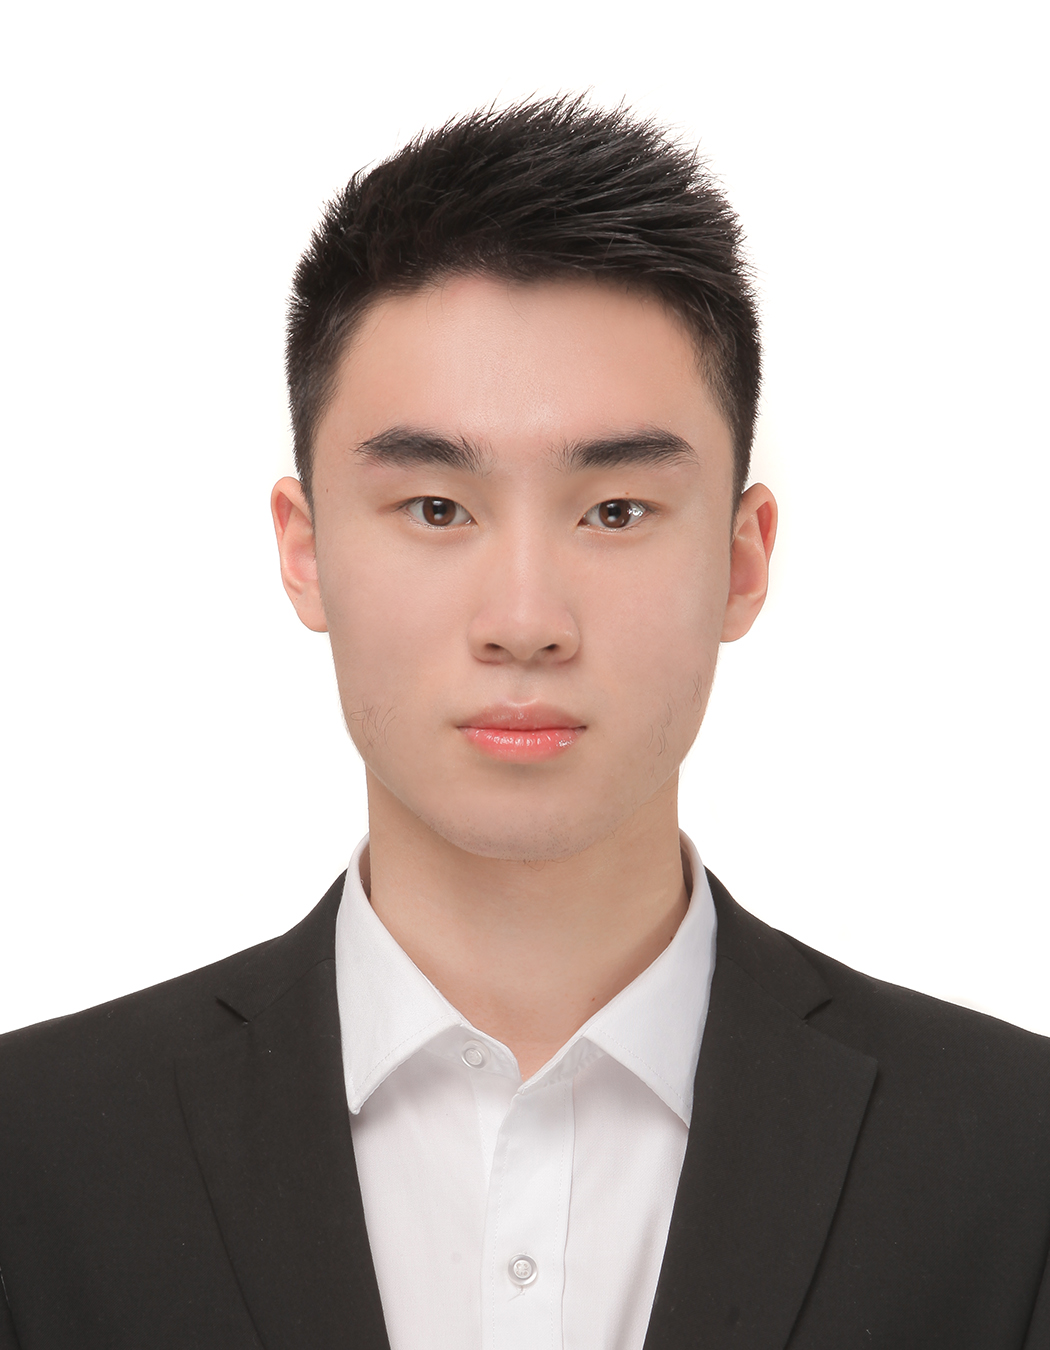
\includegraphics[width=2cm,clip]{zzy.jpg}
}
\parbox{\dimexpr\linewidth-2.8cm\relax}{
\begin{tabularx}{\linewidth}{L r} \\
  \textbf{\Large \name \nameen} & {\raisebox{0.0\height}{\footnotesize \faPhone}\ \phone}\\
  \href{mailto:\emaila}{\raisebox{0.0\height}{\footnotesize \faEnvelope}\ {\emaila}} &  \href{mailto:\emailb}{\raisebox{0.0\height}{\footnotesize \faLinkedin}\ {\emailb}}\\
  {\raisebox{0.0\height}{Major: \course}} & {\raisebox{0.0\height}{Nationality: \nationality}} \\
  {\raisebox{0.0\height}{Dob: \dob}} & {\raisebox{0.0\height}{Gender: \gender}} \\
  
\end{tabularx}
}
% \parbox{3.0cm}{%
% \flushright \includegraphics[width=2cm,clip]{nitp_logo.png}
% }




%-----------EDUCATION-----------
\section{\textbf{EDUCATION}}
  \resumeSubHeadingListStart
    \resumeSubheading
      {Shanghai Shibei Senior High School}{}
      {High Sckool Student}{2015 - 2017}
    \resumeSubheading
      {IES College}{}
      {Foundation Year Student}{2017 - 2018}
    \resumeSubheading
      {The University of Queensland}{CGPA: 3.76}
      {Bachelor of Software Engineering}{Expected June 2024}
  \resumeSubHeadingListEnd
\vspace{-5.5mm}
%



%-----------EXPERIENCE-----------------
\section{\textbf{EXPERIENCE}}
  \resumeSubHeadingListStart
    \resumeSubheading
      {The University of Queensland}{2018}
      {Back-end  developer, Chassis designer}{Brisbane}
      \vspace{-2.0mm}
      \resumeItemListStart
    \item {Developing a smart vehicle in a team. Developing a chassis that can make it keep balance while driving. Running an Arduino board. If it detected an obstacle in front of itself, it would drop a flag at the rear.}
    \resumeItemListEnd
    
    \vspace{-3.0mm}
    
    \resumeSubheading
      {The University of Queensland}{2020}
      {Volunteer}{Brisbane}
      \vspace{-2.0mm}
      \resumeItemListStart
    \item {Guiding tour of the campus for new students.。}
    
    \resumeItemListEnd
      
  \resumeSubHeadingListEnd
\vspace{-8.5mm}



%-----------PROJECTS-----------------
\section{\textbf{PROJECTS}}
\resumeSubHeadingListStart
     \resumeProject
      {Pacman} %Project Name
      {Developing a game called Pacman in a team.} %Project Name, Location Name
      {2019} %Event Dates

      \resumeItemListStart
        \item {Tools and technologies used: AVR ATmega324A microcontroller, Sensors, LED}
        \item {Role: Back-end developer\\
        The AVR ATmega324A microcontroller ran the program and received input from several sources and displayed output to a serial terminal. Implementing functions such as splashing screen, movement of pacman and eating pacdots.}
    \resumeItemListEnd
    \vspace{-2mm}
     \resumeProject
      {Fmart} %Project Name
      {Developing an online shopping app in a team. The app is helpful for stagnant fruits} %Project Name, Location Name
      {2021} %Event Dates

      \resumeItemListStart
        \item {Tools and technologies used: Adobe XD, React Native}
        \item {Role: UI designer, conducting user test and speech \\
        Working closely with front-end developer periodically to assure that design goals  can  be  achieved.  Designing interfaces that value visibility, freedom, consistency, recognition and flexibility.}
    \resumeItemListEnd
    \vspace{-2mm}
     \resumeProject
      {Smart pillow} %Project Name
      {Developing a smart pillow in a team. The product is helpful for maintaining long distance relationship.} %Project Name, Location Name
      {2022} %Event Dates

      \resumeItemListStart
        \item {Tools and technologies used: Arduino, Sensors, LED, Pillow}
        \item {Role: Project manager, conducting user test and speech\\
        Developing a rigorous project schedule. Gathering many meaningful results from the questionnaires and interviews. Designing a portion of the PowerPoint explaining the group's goals, design process, and future plans.}
    \resumeItemListEnd
    \vspace{-2mm}
  \resumeSubHeadingListEnd
\vspace{-5.5mm}



%-----------Technical skills-----------------
\section{\textbf{TECHNICAL SKILLS AND INTERESTS}}
 \begin{itemize}[leftmargin=0.05in, label={}]
    \small{\item{
     \textbf{Languages}{: Mandarin(Mother Tongue), English(IELTS: 6.0), Japanese(N2)} \\
     \textbf{Developer Tools}{: Python, HTML, CSS and JavaScript} \\
     \textbf{Framework}{: Design Framework: Design For Location Dependence} \\
     \textbf{Github}{: https://github.com/Joker1581} \\
     \textbf{Soft Skills}{: Programming, UI design} \\
     \textbf{Areas of Interest}{: Front-end developer, UI designer} \\
    }}
 \end{itemize}
 \vspace{-5mm}
 

%-----------Achievements-----------------

\section{\textbf{ACHIEVEMENTS}}
\vspace{-0.4mm}
\resumeSubHeadingListStart
\resumePOR{Xinzhi Cup Third Prize } % Award
    {Junior High School  Math Competition} % Event
    {2014} %Event Year
\resumeSubHeadingListEnd
\vspace{-5mm}
%-----------Hobbies-----------------
%\section{\textbf{Hobbies}}
%\vspace{-0.4mm}
%\resumeSubHeadingListStart
%\item Billiards, darts, swimming, tennis, singing
%\resumeSubHeadingListEnd
%-------------------------------------------
\end{document}
